% !TEX root = ../../../main.tex
% 来源：中学数学实验教材·第三册（高中数学）
% 章节：任意角的三角函数 / 三角函数的诱导公式
% 原始文件：6.tex，行 2050-2062
% 类型：tikz
% ---
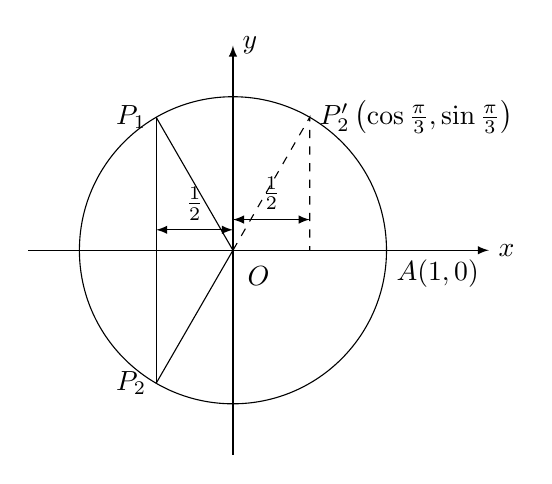
\begin{tikzpicture}[>=latex, scale=1.3]
    \draw[->](-2,0)--(2.5,0)node[right]{$x$};
    \draw[->](0,-2)--(0,2)node[right]{$y$};
    \draw (0,0) circle(1.5);
\draw (-.75, .75*1.732)node[left]{$P_1$}--(-.75, -.75*1.732)node[left]{$P_2$};
\draw (0,0)-- (120:1.5);
\draw (0,0)-- (-120:1.5);
\draw[dashed] (0,0)-- (60:1.5)node[right]{$P_2'\left(\cos\frac{\pi}{3},\sin\frac{\pi}{3}\right)$}--(.75,0);
\node at (2,0)[below]{$A(1,0)$};
\node at (.25,-.25){$O$};
\draw[<->](0,.3)--node[above]{$\frac{1}{2}$}(.75,.3);
\draw[<->](0,.2)--node[above]{$\frac{1}{2}$}(-.75,.2);
\end{tikzpicture}
